\documentclass[12pt,a4paper]{report}
\usepackage[latin1]{inputenc}
\usepackage[spanish,es-tabla]{babel}
\usepackage{graphicx}
\usepackage[left=3cm,right=3cm,top=2.5cm,bottom=2.5cm]{geometry}
\usepackage{lastpage}
\usepackage{fancyhdr}
\pagestyle{fancy}
\fancyhead[R]{\textbf{\thepage/\pageref{LastPage}}}
\renewcommand{\headrulewidth}{0pt}

\begin{document}
\begin{titlepage}
\begin{center}
\vspace*{1.5cm}
\textbf{Escuela de Ingenier��­a en Electronica}\\[0.8cm]
\textbf{Laboratorio de Dise�o de Sistemas Digitales}\\[1cm]
\textbf{Bit�cora}\\[2cm]
\textbf{Proyecto:}\\[0.4cm]
Control y programaci�n RTC con Nexys3 \\[1.7cm]
\textbf{Profesor:}\\[0.4cm]
Alfonso Chac�n Rodr��­guez \\[1.7cm]
\textbf{Estudiantes:}\\[0.4cm]
Keylor Mena Venegas \\[0.8cm]
Luis Leon Vega \\[0.8cm]
Luis Merayo Gatica \\[1.7cm]
\textbf{Periodo}\\[0.8cm]
II Semestre, 2016\\
\end{center}
\end{titlepage}


\section*{\textit{Descripci�n del problema}}

Se debe realizar un controlador para realizar la lectura y escritura del m�dulo RTC V3023. Los datos del sistema deben poder ser desplegados en un monitor LCD mediante el protocolo VGA. Ante ello, se debe realizar un controlador para el RTC y para la VGA. Asimismo, se deben poder ajustar la hora, activar la alarma y el cron�metro de forma descendente mediante botones e interruptores dispuestos en la FPGA Nexys3.

\section*{\textit{Introducci�n al proyecto}}

Este proyecto consiste en realizar un controlador de m�dulos RTC (Real Time Controller), espec��ficamente para el m�dulo V3023. Este controlador ser� capaz de escribir y leer dicho m�dulo para obtener par�metros de reloj, cron�metro y alarma. \\
Asimismo, para poder desplegar la informaci�n relevante de los par�metros anteriores, se conectar� un monitor LCD mediante el protocolo VGA. Por otro lado, para poder programar y dar instrucciones al circuito, se deber�n usar los botones se�alados en el instructivo y algunos interruptores. \\
Finalmente, el conjunto es un circuito que permita controlar el m�dulo y comunicar al usuario mediante los botones y el monitor LCD, donde �l podr� recibir la informaci�n relevante y poder modificar dicha informaci�n.\\

\section*{\textit{Objetivo General}}
Dise�ar un controlador de RTC que permita leerlo y programarlo mediante una interfaz de usuario consistente en botones incorporados dentro de la FPGA (Nexys3) y un monitor comunicado a trav�s del protocolo VGA.

\section*{\textit{Objetivos Espec��ficos}}
\begin{itemize}
	\item Investigar el funcionamiento del m�dulo RTC y el protocolo de comunicaci�n del mismo.
	\item Dise�ar un controlador para el m�dulo RTC, cuyo bus de datos y direcciones est�n multiplexados.
	\item Cumplir con las reglas de temporizado del sistema, en especial, con el protocolo de comunicaci�n del m�dulo RTC.
	\item Combinar el controlador de RTC con un controlador VGA para poder desplegar la informaci�n del m�dulo al usuario. Este m�dulo VGA ser� adaptado del proyecto anterior.
	\item Desarrollar un banco de pruebas (testbench) para poder emular el comportamiento del m�dulo RTC con la finalidad de comprobar el funcionamiento del circuito controlador.
\end{itemize}

\newpage

% Comienzo de la bitacora
\section*{\textit{Control de eventos}}
% Nueva entrada
\begin{flushright}
	\begin{large}
		\textbf{Fecha: 10 de Noviembre}\\[5ex]
	\end{large}
\end{flushright}

\noindent \textbf{Integrantes:} todos \\[1ex]
\textbf{Hora:} 20:00 -22:30 pm \\[1ex]
\textbf{Actividad:} \\[2ex]
Se dise�o el primer intento de aproximarse a un diagrama de bloques de nivel 2. Esto se puede notar en la figura \ref{fig:DigramaNivel2.1}, en este se puede notar 5 bloques principales, uno de ellos es el microprocesador echo con el picoblaze. Ademas podemos notar que este tiene como entrada las se�ales PosX y PosY de la VGA, de esta manera se controla la lectura de la RTC cuando la VGA se encuentra pintando en algunos lugares de la pantalla, Ademas la entrada IRQ controla cuando la etapa de sonido funciona.\\
La memoria alimenta con los datos que debe pintar la VGA, estos datos vienen de la RTC directamente cuando se encuentra actualizando los datos. ademas que posee un espacio para la se�al IRQ y el teclado.\\
El teclado introduce a la memoria los datos que el usuario desea cambiar para que se muestre inmediatamente en la VGA. Ademas una vez que el usuario desea introducir el cambio en la RTC, este bloque se comunica con el controlador RTC para introducir el cambio.\\
 

\begin{figure}[hbtp]
	\centering
	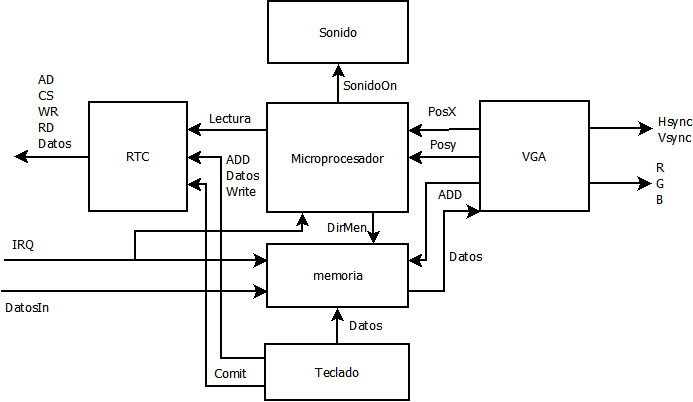
\includegraphics[width=14cm]{Img/Digrama_tercer_proyecto.png}
	\caption{Diagrama de bloques nivel 2 primer intento}
	\label{fig:DigramaNivel2.1}
\end{figure}




\end{document}